
\chapter{Evaluation\label{evaluation}}

This chapter discusses how the changes implemented in chapter \ref{improvements} impact the performance of RIR.

For evaluation, the Shootout benchmarks were used (see \autocite{fastr, shootout}). These are small programs that focus on different parts of R, such as recursive calls, loops, vector arithmetic, string manipulation etc. The details are in table \ref{tab:shootout}, taken from \autocite{fastr}.

\begin{longtable}[c]{@{}ll@{}}
\caption{The Shootout benchmark suite\label{tab:shootout}} \tabularnewline
\toprule
Benchmark & Description \tabularnewline
\midrule
\endfirsthead
\toprule
Benchmark & Description \tabularnewline
\midrule
\endhead
binarytrees & Allocates and traverses binary trees \tabularnewline
& \emph{GC benchmark, recursive calls, recursive lists} \tabularnewline
fannkuchred & Solves a combinatorial problem \tabularnewline
& \emph{Loops, indexing short vectors} \tabularnewline
fasta & Generates DNA sequence by copying, rand. selection \tabularnewline
& \emph{String operations, scalar arithmetic} \tabularnewline
fastaredux & Solves same problem as fasta \tabularnewline
& \emph{Adds more loops, vector indexing and arithmetic} \tabularnewline
knucleotide & Finding patterns in gene sequences \tabularnewline
& \emph{Uses environment as a hashmap, string operations} \tabularnewline
mandelbrot & Calculates a Mandelbrot set (fractal image) \tabularnewline
& \emph{Vector arithmetic on complex numbers} \tabularnewline
nbody & Solves the N-body problem (simulation) \tabularnewline
& \emph{Arithmetic, Math with short vectors} \tabularnewline
pidigits & Calculate digits of pi using spigot algorithm \tabularnewline
& \emph{Arbitrary precision arithmetic in R (diverse code)} \tabularnewline
regexdna & Matching, replacing regex-specified gene sequences \tabularnewline
& \emph{Regular expressions (falls back to regex library)} \tabularnewline
reversecompl & Computing reverse-complements for gene sequence \tabularnewline
& \emph{String vector indexing using string names} \tabularnewline
spectralnorm & Computing eigenvalue using power method \tabularnewline
& \emph{Loops, function calls, scalar arithmetic} \tabularnewline
\bottomrule
\end{longtable}

The benchmark problems come from The Computer Language Benchmarks Game.\footnote{See \url{http://benchmarksgame.alioth.debian.org/}.} The R language mutation was added by Leo Osvald \autocite{shootout}. There are several versions of most problems, the naive ones being more or less a literal translation from C or Java to R. The alternative implementations solve the same problems, however, they use different styles of programming that leverage various features available in R, as experienced R programmers would.

The benchmarks were run on a machine with \emph{Intel(R) Core(TM) i5-6500} (4 cores) and 8~GB of memory. For every benchmark, three experiments were measured: GNU R interpreted code (JIT set to 0), GNU R byte-compiled code (JIT set to 2 and optimize to 2) and RIR compiled code (JIT set to 2).

Each experiment took place in a fresh R session. The benchmark code was sourced, then it was executed 12 times, and the last 8 measured times were logged. This ensured that the machine was warmed up properly. Any compile time overheads were disregarded. The same measurements were performed for every set of added features.

Figure \ref{fig:overall} shows the summary of how much the difference between RIR and GNU R was lowered for each benchmark, as well as an overall average (smaller values are better).

\begin{figure}[htbp]
  \caption{\label{fig:overall}Overview of the slowdowns vs. GNU R}
  \centering
  \tmpframe{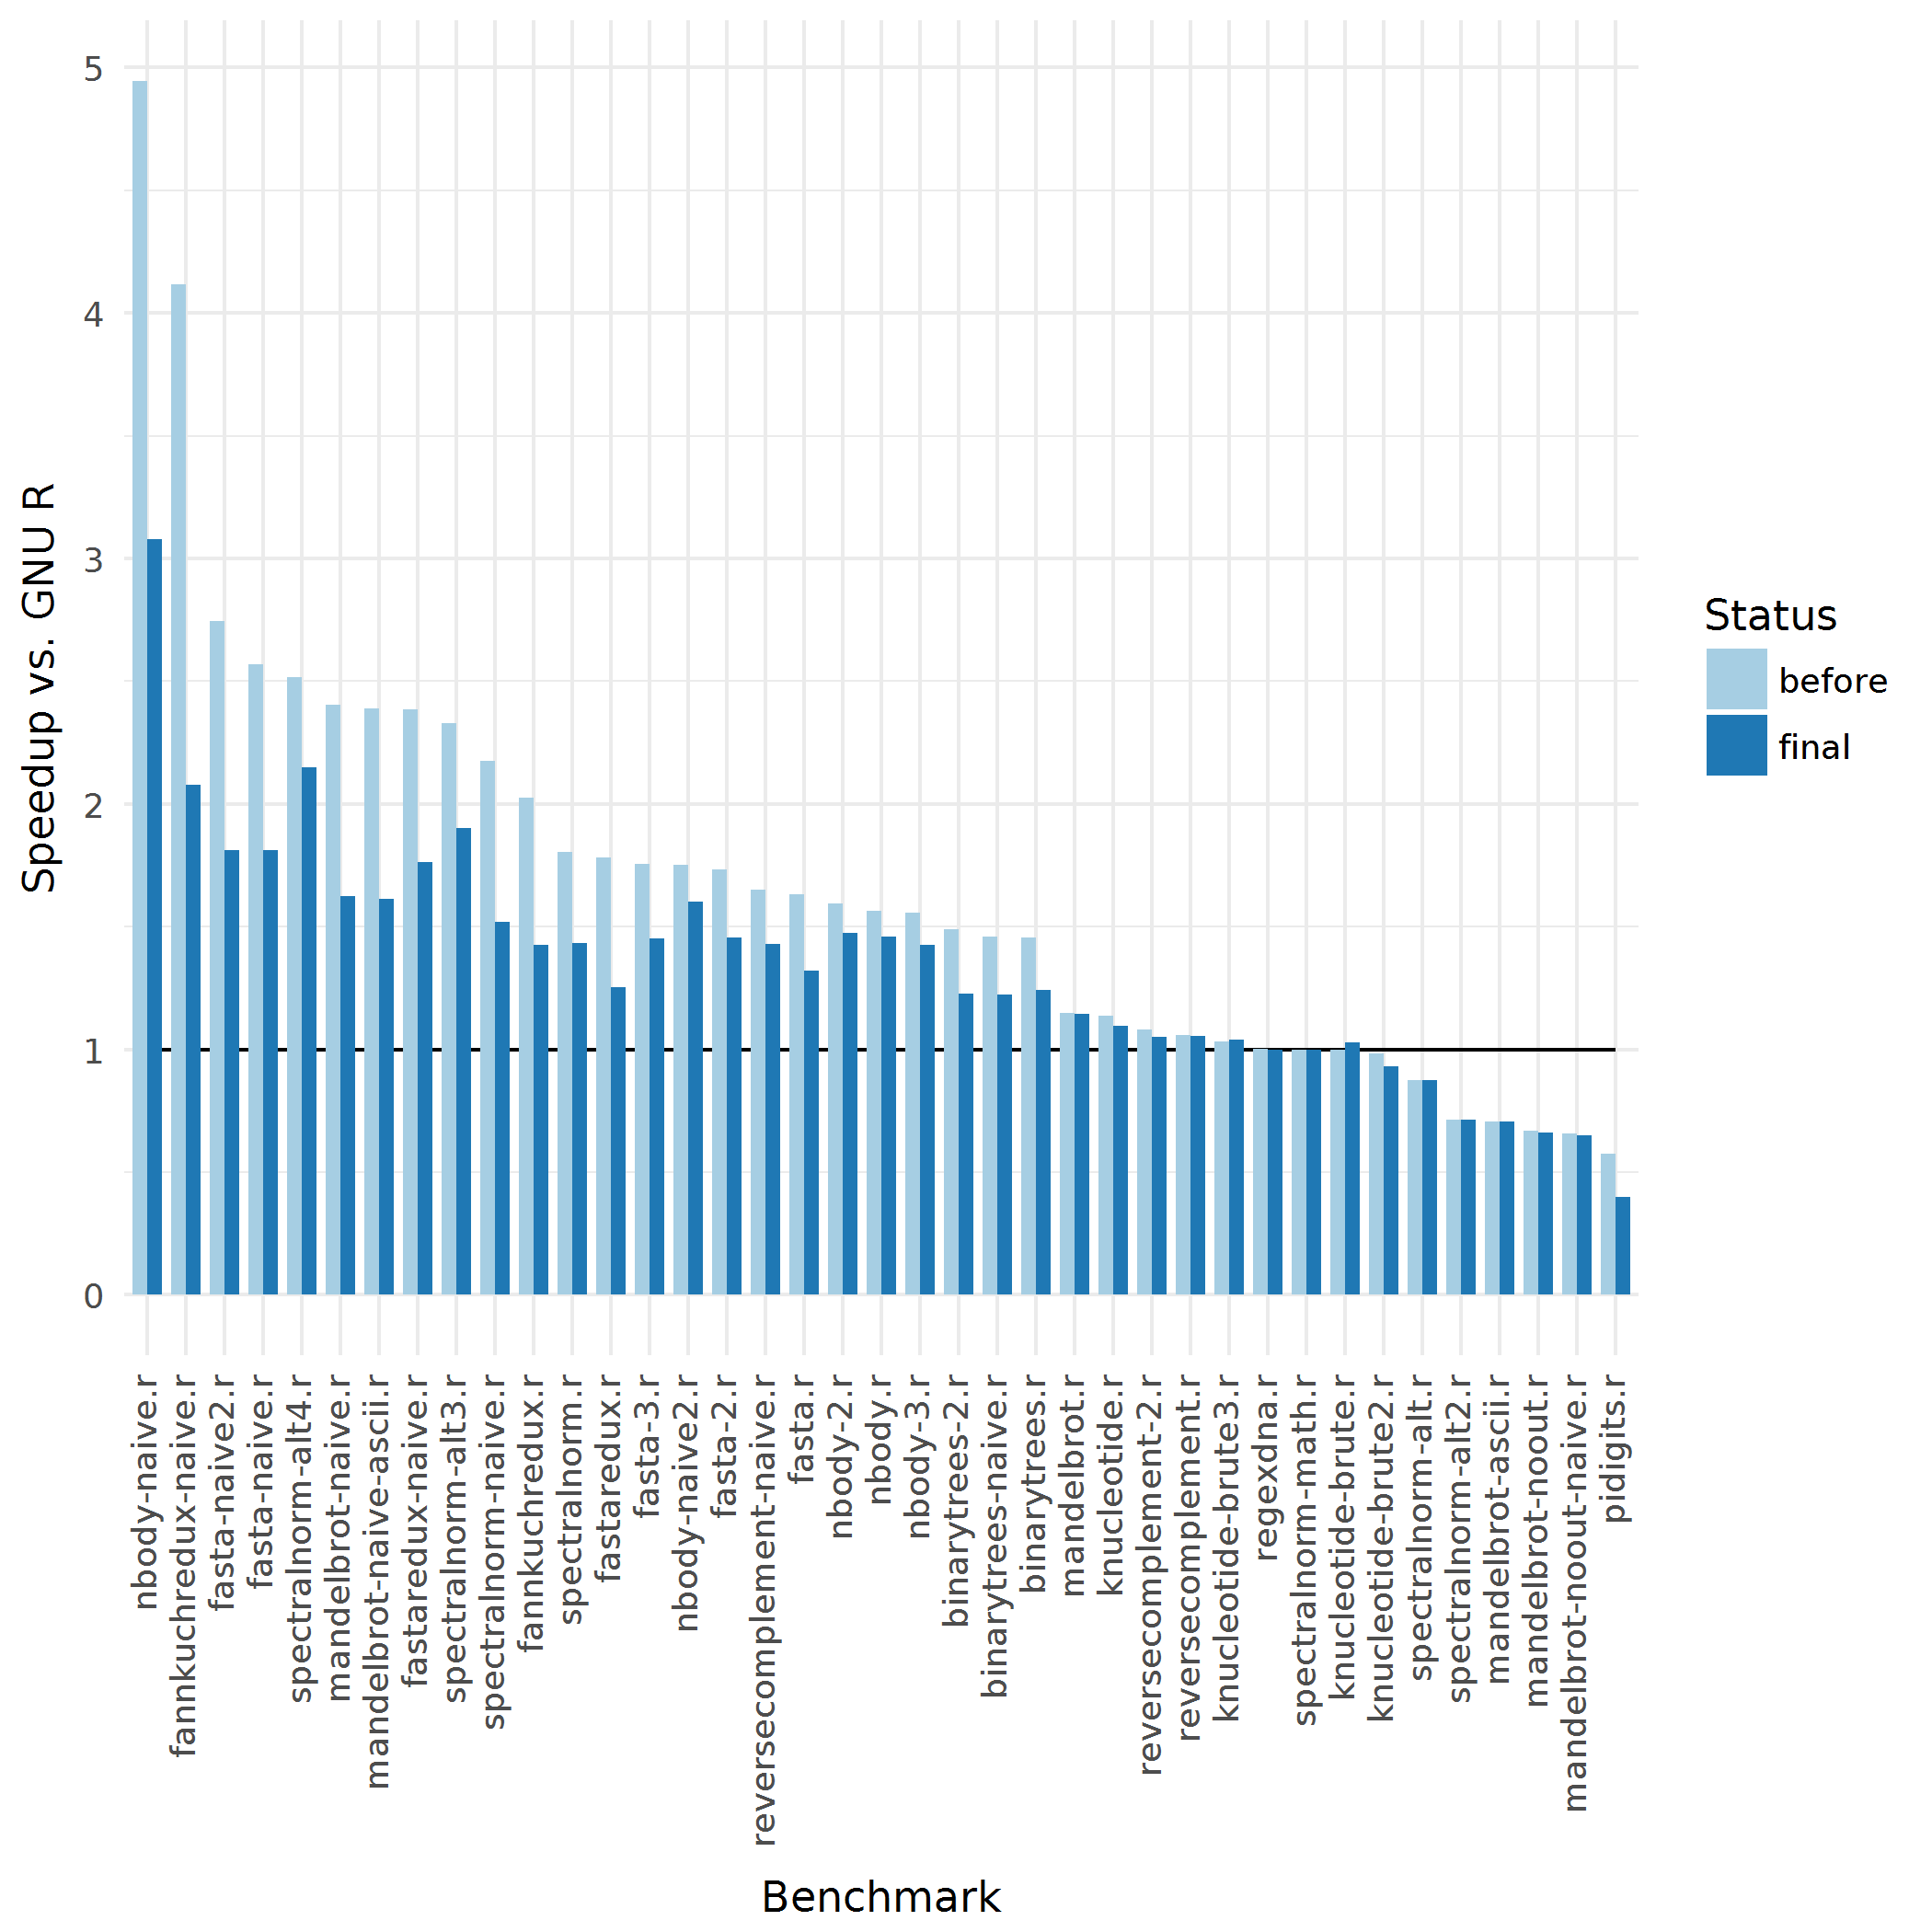
\includegraphics[width=\linewidth]{images/overall}}
\end{figure}

The lighter color refers to the state before any feature was added, the darker after all the changes described in chapter \ref{improvements}.

The slowdowns are computed relative to the running time of GNU R byte-compiled code, which was normalized to 1 (and is indicated by the solid black line).

Overall, an average slowdown against GNU R was lowered by about 50~\% (from a factor of 1.678 to 1.336).

It can be clearly seen that the most speedup was gained for the naive versions of benchmarks. These are the programs that use a lot of nested loops, lot of arithmetic operations and have relatively long functions, which is exactly the area where the efforts of chapter \ref{improvements} were focused.

The revisions that were used to monitor the progress, together with their features, are listed in table \ref{tab:git-rev}. The table also shows the average speedup over all benchmarks of each feature set, relative to the first revision.

\begin{longtable}[c]{@{}llc@{}}
\caption{Git revisions used in the benchmarks\label{tab:git-rev}} \tabularnewline
\toprule
Hash & Features & Avg. speedup \tabularnewline
\midrule
\endfirsthead
\toprule
Hash & Features & Avg. speedup \tabularnewline
\midrule
\endhead
e1091b9 & State before the first changes & 1.0 \tabularnewline
594af0c & Added relational and unary operators & 1.029 \tabularnewline
ce30085 & Loop contexts removal & 1.043 \tabularnewline
6c4f526 & BC cleanup and colon operator & 1.054 \tabularnewline
f8e8238 & Superassignment operator & 1.081 \tabularnewline
12ef757 & Interpreter loop refactoring & 1.199 \tabularnewline
ff73d75 & Use indirect threading & 1.206 \tabularnewline
\bottomrule
\end{longtable}

Figure \ref{fig:history} captures the running times of each benchmark over the course of the work described in chapter \ref{improvements}.

\begin{figure}[htbp]
  \caption{\label{fig:history}History of running times}
  \centering
  \tmpframe{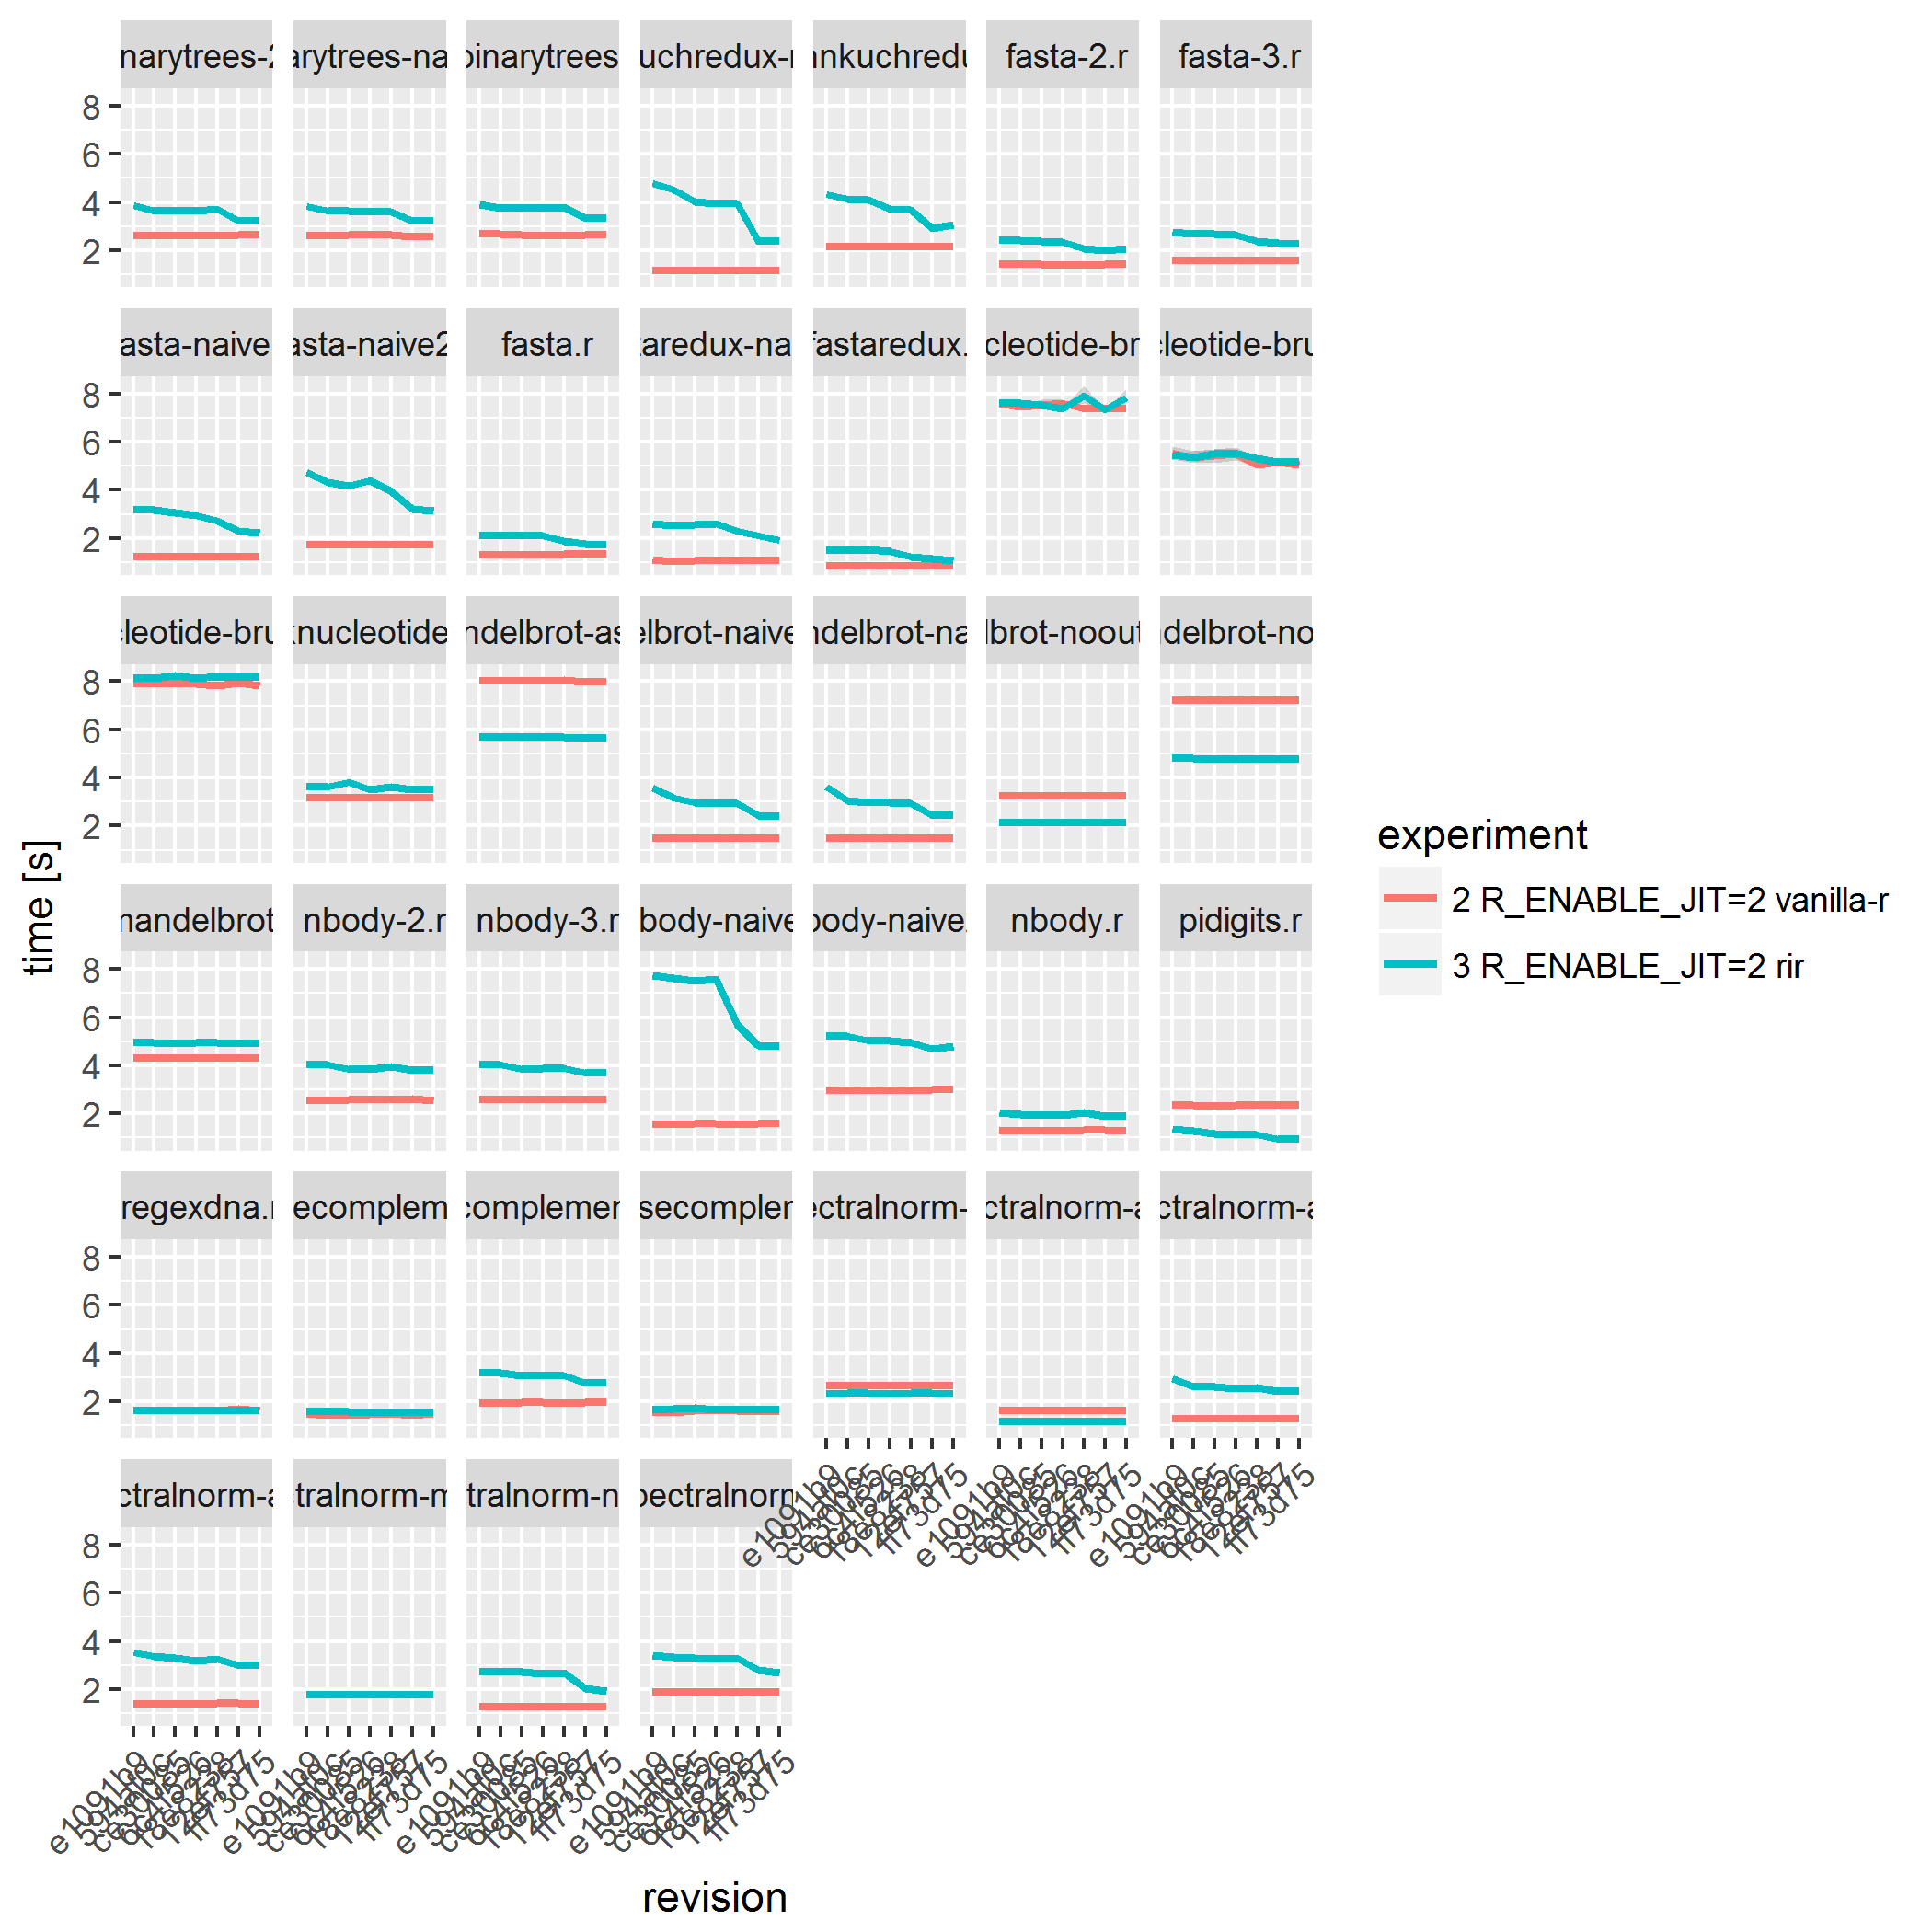
\includegraphics[width=\linewidth]{images/speedup_history}}
\end{figure}

In the figure, the light blue color represents performance of the GNU R bytecode. As all measurements were carried out on the same version of GNU R (namely 3.3.2) the times are identical.

RIR performance for some benchmarks was comparable to GNU R even before the first modifications, with some (notably \emph{pidigits}) outperforming GNU R. In particular, the \emph{pidigits} code is the longest of the benchmarks (in terms of lines of code), has a lot of user-defined functions and seems to spend most of the time executing the bytecode. Together with the \emph{mandelbrot} versions where RIR is faster that do mostly just arithmetic in loops, this suggests that when there are few calls into plain R and all work is done in the bytecode interpreters, RIR is competitive.

Other benchmarks have remained more or less constant throughout. This is because they do not use that much bytecode instructions and instead spend the majority of time inside builtin C code. Therefore changes to the bytecode have almost no effect on them.

Generally, the biggest improvements were brought by inlining the instructions into the interpreter loop. With the exception of some benchmarks not affected by any changes, all others gained a boost. The nature of this change is such that it speeds up every bytecode instruction a tiny bit. Thus all benchmarks that spend some considerable time in the bytecode interpreter see an improvement.

For some benchmarks, a particular revision brings minor slowdowns. The reasons are not entirely clear and require some more investigation. For instance, an operator that checks a fast path and then falls back to the builtin call anyway may be slower than calling the builtin directly. On the other hand, taking into consideration branch prediction in the CPU and the fact that the call instruction has some overhead too (e.g., for preparing the argument list), this seems unlikely.

Two of the benchmarks were rerun with 20 iterations and their plots then zoomed to present a more detailed view. These were \emph{nbody naive}, to show the steep bump, and \emph{knucleotide brute}, because it originally had very wide confidence intervals. This suggested that perhaps the CPU was loaded by some other work during the original measurements.\footnote{Unfortunately, rerunning all of the benchmarks was not possible due to time constraints on the test server.}

The detailed view of the \emph{nbody naive} benchmark is in figure \ref{fig:nbody}. The benchmark gained the most with inlining superassignment, as it uses it heavily in nested loops. Another large speedup was due to the interpreter refactoring and is so distinctive because the produced bytecode for the main hotspot (the function \rinline/advance/) is very arithmetic heavy with a lot of loops and subsetting and few calls. This means that long sequences of instructions get executed at once, thus leveraging the improved interpreter loop.

\begin{figure}[htbp]
  \caption{\label{fig:nbody}Detail of the \emph{nbody naive} benchmark}
  \centering
  \tmpframe{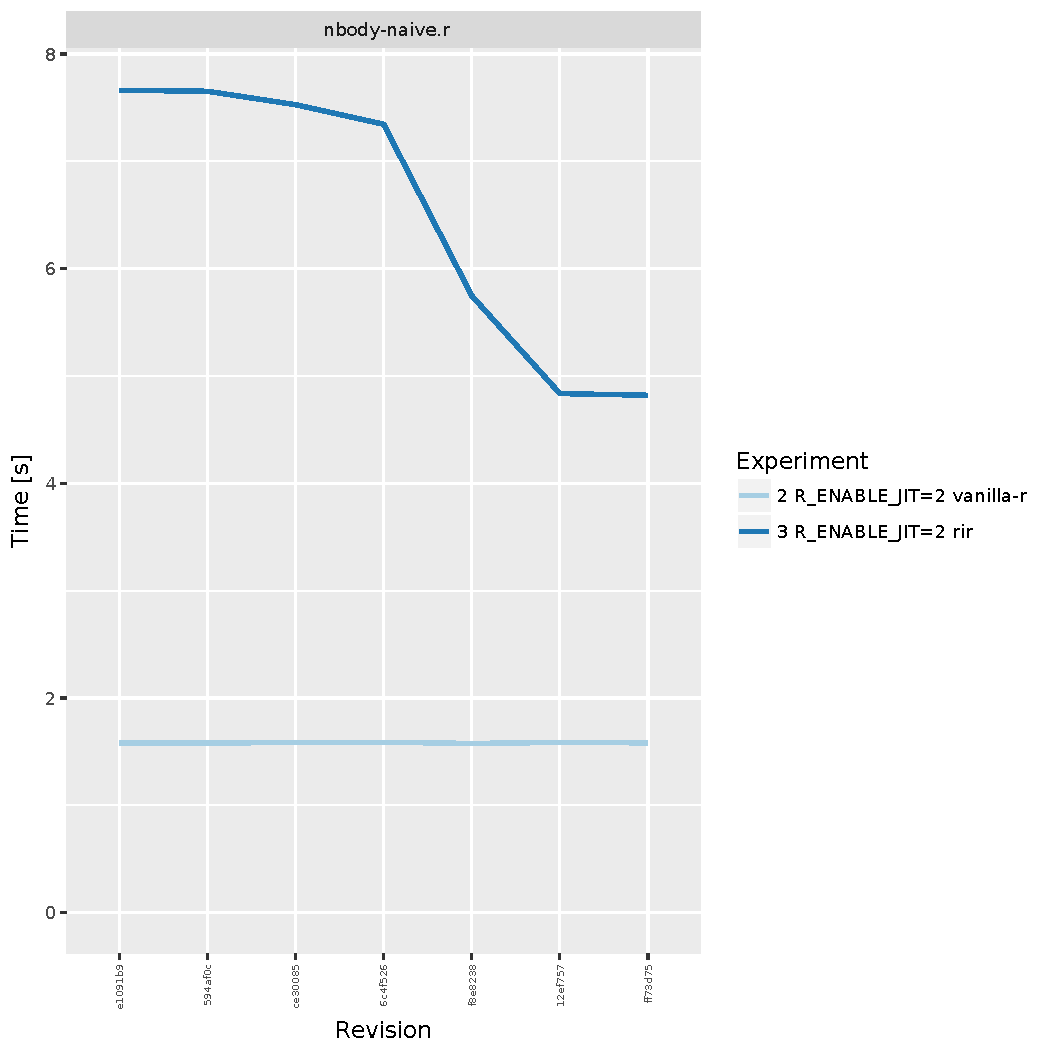
\includegraphics[width=0.495\linewidth]{images/nbody-naive}}
\end{figure}

As for the \emph{knucleotide brute} benchmark in figure \ref{fig:knucleotide}, the confidence intervals were indeed a byproduct of the CPU load and disappeared after the rerun. However, there are still some inexplicable fluctuations for the GNU R version, which will require future investigation.

\begin{figure}[htbp]
  \caption{\label{fig:knucleotide}Detail of the \emph{knucleotide brute} benchmark}
  \centering
  \tmpframe{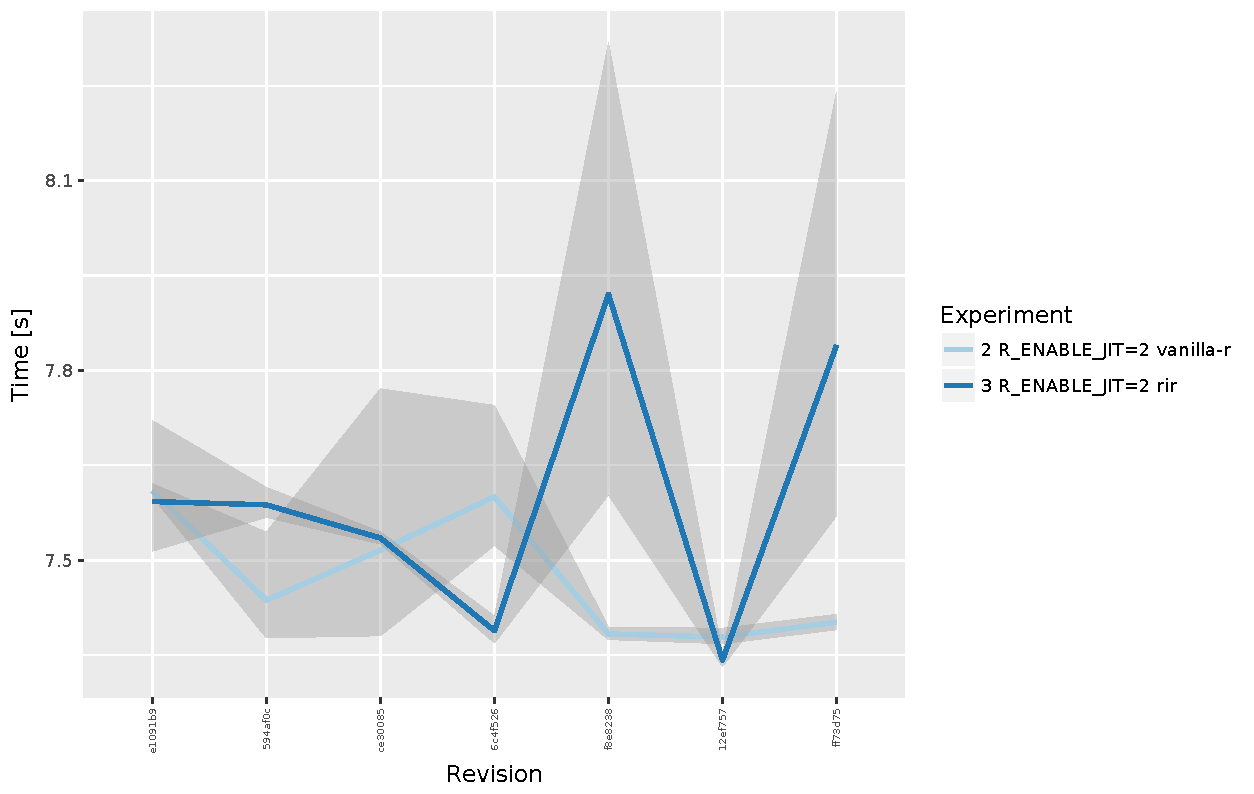
\includegraphics[width=0.495\linewidth]{images/knucleotide-brute}}
\end{figure}

The average speedup versus GNU R over the measured revisions is captured in figure \ref{fig:avg-speedup-history}. The result was obtained by averaging the measurements for each benchmark and then taking the average of those values. Of the changes, the most debatable is threading. It seems that this feature only starts to pay off for larger and longer programs.

\begin{figure}[htbp]
  \caption{\label{fig:avg-speedup-history}History of average speedup vs. GNU R}
  \centering
  \tmpframe{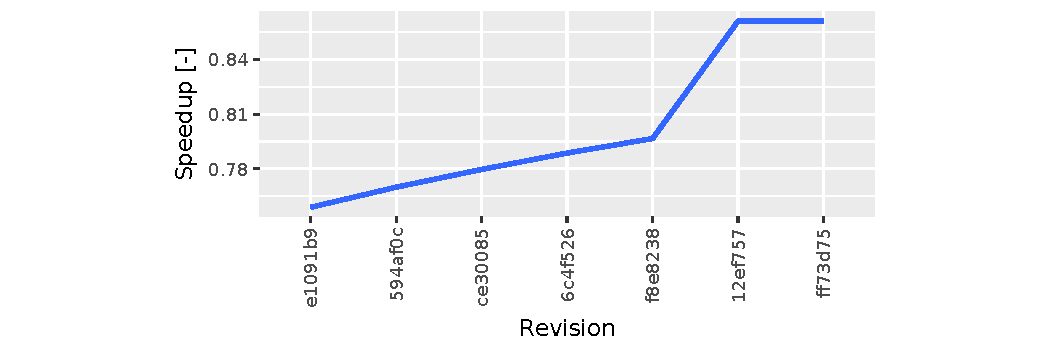
\includegraphics[width=\linewidth]{images/avg_speedup}}
\end{figure}
